%%%%%%%%%%%%%%%%%%%%%%%%%%%%%%%%%%%%%%%%%%%%%%%%%%%%%%%%%%%%%%%
%
% Open Research Europe is an open access publishing platform for the publication of research stemming from Horizon 2020 funding across all subject areas. The platform makes it easy for Horizon 2020 beneficiaries to comply with the open access terms of their funding and offers researchers a publishing venue to share their results and insights rapidly and facilitate open, constructive research discussion.
%
%%%%%%%%%%%%%%%%%%%%%%%%%%%%%%%%%%%%%%%%%%%%%%%%%%%%%%%%%%%%%%%
%
% This template is for all article types; for information on specific article type requirements please visit https://open-research-europe.ec.europa.eu/for-authors/article-guidelines
%
% For more information on the Open Research Europe publishing model please see:  https://open-research-europe.ec.europa.eu/about

\documentclass[10pt,a4paper]{article}
\usepackage{f1000_styles}

%% Default: numerical citations
\usepackage[numbers]{natbib}
% defines Environment longtable
\usepackage{longtable}
\usepackage{booktabs}
%% Uncomment this lines for superscript citations instead
% \usepackage[super]{natbib}

%% Uncomment these lines for author-year citations instead
% \usepackage[round]{natbib}
% \let\cite\citep

% fix figures
\let\oldincludegraphics\includegraphics
\renewcommand{\includegraphics}[2][]{\oldincludegraphics[width=0.8\textwidth,#1]{#2}}

% remove numbering
\setcounter{secnumdepth}{-\maxdimen} % remove section numbering

\begin{document}
\pagestyle{fancy}

\title{Assessing the validity of a calcifying oral biofilm model as a
suitable proxy for dental calculus}
%\titlenote{Please provide a concise and specific title that clearly reflects the content of the article.}

\author[]{
Bjørn Peare Bartholdy,
Irina M. Velsko,
Shira Gur-Arieh,
Zandra Fagernäs,
Christina Warinner,
Amanda G. Henry}
\affil[]{
Faculty of Archaeology, Leiden University\\
\\Department of Archaeogenetics, Max Planck Institute for Evolutionary
Anthropology\\
\\The Leon Recanati Institute for Maritime Studies, University of
Haifa\\
Institute of Pre- and Protohistoric Archaeology, University of Kiel\\
\\Department of Archaeogenetics, Max Planck Institute for Evolutionary
Anthropology\\
Globe Institute, University of Copenhagen\\
\\Department of Anthropology, Department of Anthropology, Harvard
University\\
Department of Archaeogenetics, Max Planck Institute for Evolutionary
Anthropology\\
\\Faculty of Archaeology, Leiden University\\
}

% \author[1]{Author Name-1}
% \author[2]{Author Name-2}
% \affil[1]{Address of author-1}
% \affil[2]{Address of author-2}

\maketitle
\thispagestyle{fancy}


\begin{abstract}

Dental calculus is increasingly used by researchers to study dietary
patterns in past populations. The benefits of using dental calculus for
this purpose have been clearly demonstrated in previous studies, with
dental calculus harbouring a wealth of microremains and biomarkers for
health and diet within its mineral matrix. Previous studies have
demonstrated some of the limitations and biases of how methods of
processing may overlook, or even remove, some of the important
information contained within the mineralised matrix. However, there are
many factors that are impossible to account for \emph{in vivo} and in
archaeological material, such as exact dietary intake, and individual
factors such as pH and enzyme activity, leaving some limitations that
may not be addressed through these types of studies and will require a
different approach.

We present a protocol for creating a calcifying oral biofilm model that
can be used to explore the biases and limitations of dental calculus as
a medium for paleodietary reconstructions. We report the microbial and
mineral composition of our model in an effort to validate the model
calculus as an appropriate proxy to natural dental calculus. The
microbial profile and species diversity of our model was determined
using metagenomic classification with the nf-core/eager pipeline and
Kraken2, and compared to various reference samples from oral sites,
including saliva, plaque, and dental calculus. We then assessed whether
our model calculus mineralises in a manner similar to natural dental
calculus using Fourier transform infrared (FTIR) spectroscopy. The
metagenomic classification showed a microbial profile predominantly made
up of (facultative) anaerobes, with a community structure that was
somewhat distinct from other oral reference samples. The core genera of
the model consisted of oral species, but clustered separately from oral
reference samples, with a higher abundance of anaerobes.\\
Mineral and organic components of our model mimic that of the modern and
archaeological reference calculus that was used as a comparison. There
was an overall increase in the inorganic component relative to organic
over the course of the experiment, with carbonated hydroxyapatite as the
principal compound, consistent with natural human-derived calculus.

We conclude that oral biofilm models, such as the one presented in this
study, have great potential to validate current methods used in the
analysis of archaeological dental calculus, and should be used to
complement, rather than replace current \emph{in vivo} studies.

\end{abstract}

\section*{\color{OREblue}Keywords}

oral biofilm, dental calculus, microbiome, metagenomics, ftir



\clearpage
\pagestyle{fancy}

\section*{Plain language summary}

Archaeologists have been using dental calculus (or tartar) for many
decades to find traces of food from the past. What makes dental calculus
so well suited for this task is that it forms on our teeth, and is
therefore in direct contact with what we eat. It also hardens to form a
strong, solid material that can survive for long periods of time and
preserve what's inside. While we have been able to extract a lot of
information from archaeological dental calculus, there are still many
things we don't know about the context of this information. For example,
we have no way to confirm exactly what people were eating, we can only
infer this from what we see; but, there are many factors that influence
what actually ends up in dental calculus, and it's not all food.

To address some of these issues, we have grow our own dental calculus in
a lab under controlled conditions. This will allow us to conduct
experiments to test what we see and how it relates to the
interpretations we make. In this study, we examine our lab-grown dental
calculus to make sure it looks and behaves like naturally-occurring
dental calculus, specifically the bacterial and mineral content. We
found some differences in bacterial content, which is not uncommon for
lab-grown dental plaque and calculus. Overall, though, the lab-grown
model has the makeup of an oral microbiome, and the mineral content is
very similar to natural dental calculus.

We recommend using lab-grown models to mitigate some of the issues we
encounter when using archaeological dental calculus to reconstruct past
diets, while we also acknowledge that the model is not a replacement for
research on natural calculus, both archaeological and modern.

\newcommand{\pandocbounded}[1]{#1}

\section{Introduction}\label{introduction}

Dental calculus is becoming an increasingly popular substance for
exploring health and diet in past populations
\citep{warinnerNewEra2015}. During life, dental plaque undergoes
periodic mineralisation, trapping biomolecules and microfossils that are
embedded within the dental plaque biofilm in the newly-formed dental
calculus. This process is repeated as new plaque is deposited and
subsequently mineralises, resulting in a layered structure representing
a temporal record of biofilm growth and development
\citep{warinnerPathogensHost2014}. The calculus serves as a protective
casing for the entrapped biomolecules and microfossils, preserving them
for thousands of years after death and burial
\citep{yatesOralMicrobiome2021}. Studies using archaeological dental
calculus span a wide range of topics in different regions and time
periods. These include characterisation of the oral microbiome and its
evolution in past populations
\citep{velskoMicrobialDifferences2019, adlerSequencingAncient2013, warinnerPathogensHost2014, kazarinaPostmedievalMicrobial2021, yatesOralMicrobiome2021},
as well as extraction of microbotanical remains
\citep{henryCalculusSyria2008, hardyStarchGranules2009, mickleburghNewInsights2012, maHumanDiet2022}
and other residues to infer dietary patterns and nicotine use
\citep{buckleyDentalCalculus2014, hendyProteomicCalculus2018, eerkensDentalCalculus2018, bartholdyMultiproxyAnalysis2023, velskoDentalCalculus2017}.
Dental calculus has already provided a unique and valuable insight into
the past, but the exact mechanism of the incorporation, retention, and
preservation of microfossils and biomolecules exogenous to the microbial
biofilm is largely unknown; even the process of plaque mineralisation is
not fully understood
\citep{omelonReviewPhosphate2013, jinSupragingivalCalculus2002}. This
means that there may be hidden biases affecting our interpretations of
dietary/activity patterns extrapolated from ancient dental calculus.
These biases have been explored archaeologically
\citep{fagernasMicrobialBiogeography2022, trompEDTACalculus2017} as well
as in contemporary humans \citep{leonardPlantMicroremains2015} and
non-human primates \citep{powerChimpCalculus2015}, but not
experimentally.

Dental plaque is an oral biofilm and is part of the normal state of the
oral cavity. However, when left unchecked, plaque can lead to
infections, such as dental caries and periodontitis, and/or
mineralisation \citep{marshDentalPlaque2006}. The dental plaque biofilm
grows in a well-characterized manner before mineralisation, in a process
that repeats regularly to build up dental calculus. Shortly after teeth
are cleaned (whether mechanically or otherwise), salivary components
adsorb to the crown or root and form the acquired dental pellicle. The
pellicle provides a viable surface for bacteria to attach, especially
early-coloniser species within the genera \emph{Streptococcus} and
\emph{Actinomyces} \citep{marshDentalPlaque2006}. Once the tooth surface
has been populated by specialists in surface-attachment, other species
of bacteria can attach to the adherent cells, increasing the biofilm
density and diversity. The bacterial species secrete polysaccharides,
proteins, lipids, and nucleic acids, into their immediate environment to
form a matrix that provides structural support, nutrition, and allows
for environmental niche partitioning
\citep{flemmingBiofilmsEmergent2016}.

Biofilms can become susceptible to calcification under certain
microenvironmental conditions, including an increased concentration of
salts and a decrease in statherin and proline-rich proteins in saliva,
rises in local plaque pH, and increased hydrolysis of urea
\citep{whiteDentalCalculus1997, wongCalciumPhosphate2002}. These
conditions can cause increased precipitation and decreased dissolution
of calcium phosphate salts within saliva and the plaque biofilm. The
resulting supersaturation of calcium phosphate salts is the main driver
of biofilm mineralisation \citep{jinSupragingivalCalculus2002}. The
primary minerals in dental calculus are hydroxyapatite, octacalcium
phosphate, whitlockite, and brushite. During initial mineralisation the
main mineral component is brushite, which shifts to hydroxyapatite in
more mature dental calculus
\citep{jinSupragingivalCalculus2002, hayashizakiSiteSpecific2008}. The
exact elemental composition of dental calculus varies among individuals
due to various factors, including diet
\citep{hayashizakiSiteSpecific2008, jiFluorideMagnesium2000}.

Dental plaque can also be grown \emph{in vitro}, and these oral biofilm
models are commonly used in dental research to assess the efficacy of
certain treatments on dental pathogens
\citep{filochePlaqueMicrocosm2007, extercateAAA2010} without the ethical
issues of inducing plaque accumulation in study participants and the
complexity of access and sampling in humans or animals. Oral biofilm
models are often short-term models grown over a few days, but longer
term models also exist (up to six weeks) which are used to develop
mature plaque or dental calculus
\citep{middletonVitroCalculus1965, sissonsMultistationPlaque1991, wongCalciumPhosphate2002, velskoConsistentReproducible2018}.
A well-known limitation of biofilm models is the difficulty in capturing
the diversity and complexity of bacterial communities and metabolic
dependencies, micro-environments, nutrient availability, and host
immune-responses in the natural oral biome
\citep{edlundUncoveringComplex2018, bjarnsholtVivoBiofilm2013, velskoConsistentReproducible2018, velskoCytokineResponse2017}.
These limitations can be overcome by complex experimental setups, but at
the cost of lower throughput and increased requirements for laboratory
facilities.

Despite the limitations, oral biofilm models have many benefits over
\emph{in situ} research. There are many variables involved in dental
calculus formation, such as intra- and inter-individual variation in
salivary flow, oral pH, and amylase activity, which can be hard to tease
apart \emph{in situ}. Oral biofilm models provide a controlled
environment to explore the effect of selected variables on the growth of
calculus and the retention of dietary components in the biofilm, as well
as a means to identify how the methods used in archaeology may
inadvertently bias the interpretations. This type of research has, so
far, been limited, but has the potential to greatly benefit
archaeological research on past diet \citep{radiniDirtyTeeth2022}.

We present an oral biofilm model that can serve as a viable proxy for
dental calculus for archaeology-oriented research questions. It is a
multispecies biofilm using whole saliva as the inoculate, with a simple
multiwell plate setup that is accessible even to smaller lab budgets and
those with limited facilities for microbiology work. Here, we used
next-generation sequencing and metagenomic classification to
characterise the bacterial composition of our model dental calculus and
compare it to oral reference samples, including saliva, buccal mucosa,
plaque, and modern human dental calculus. This was done to ensure that
the model microbiome is predominantly oral and not overgrown by
environmental contaminants. We then determined the mineral composition
of the model dental calculus using Fourier transform infrared (FTIR)
spectroscopy to verify the presence of calculus-specific mineral phases
and functional groups, and perform a qualitative comparison with modern
and archaeological reference calculus. Overall the model calculus is
chemically similar to natural calculus, and has a predominantly oral
microbiome. The microbial diversity and richness within the model
samples were lower than oral reference samples, suggesting that the
model samples do not contain identical species composition and
abundances as the natural samples. The mineral composition closely
resembles modern and archaeological reference calculus, predominantly
comprised of carbonate hydroxyapatite with a similar level of
crystallinity and order. As such, the model dental calculus presented
here is a viable proxy to natural dental calculus and can be used to
explore many of the currently unexplained processes we see in the
archaeological material, when working within the limitations of an oral
biofilm model.

\section{Materials and Methods}\label{materials-and-methods}

Our biofilm setup consists of whole saliva as the inoculate to
approximate natural microbial communities within the human oral cavity,
and a 24-well plate to generate multiple replicated conditions in a
single experimental run (see Figure~\ref{fig-met-protocol} for an
overview of the protocol). The biofilm is grown for 25 days to allow
time for growth of larger deposits and mineralisation. Raw potato and
wheat starch solutions were added during the biofilm growth to explore
the biases involved in their incorporation and extraction from dental
calculus. These results are presented in a separate article
\citep{bartholdyInvestigatingBiases2022}.

\begin{figure}

\centering{

\pandocbounded{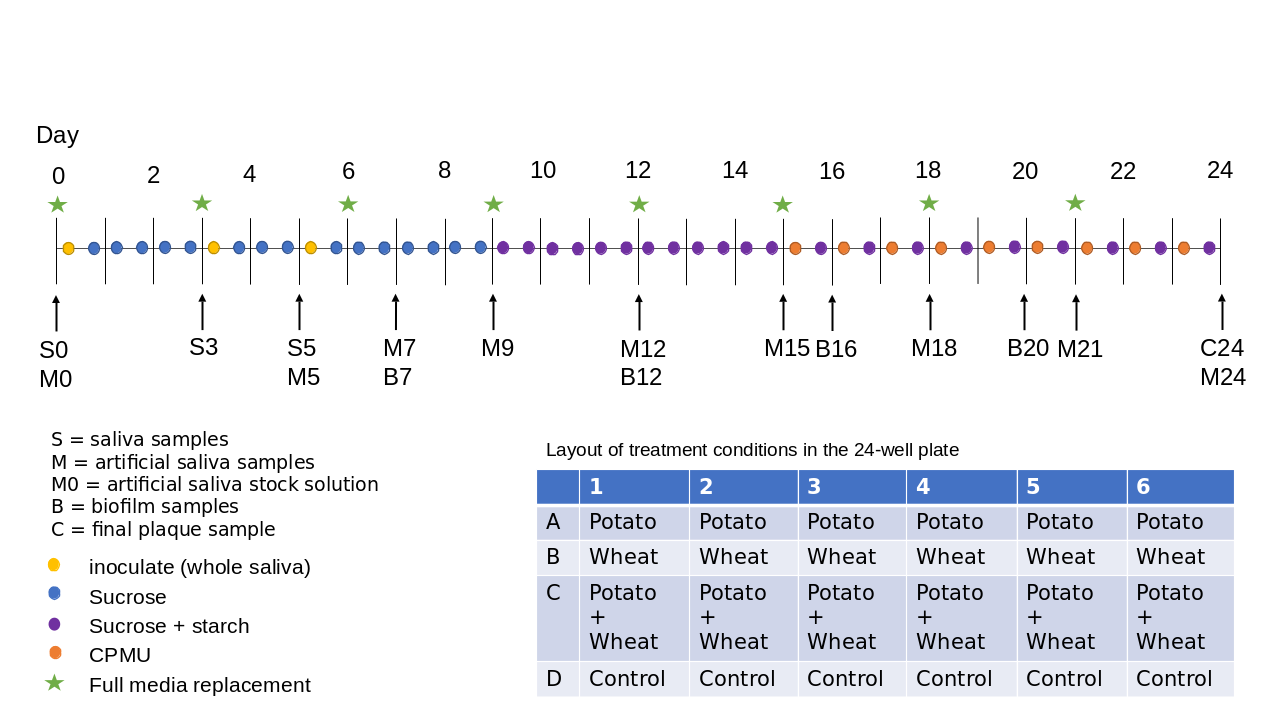
\includegraphics[keepaspectratio]{figures/Exp_protocol.png}}

}

\caption{\label{fig-met-protocol}Overview of the protocol for biofilm
growth. The samples for metagenomic analysis were grown in a separate
experimental plate than the FTIR samples under the same experimental
conditions. Biofilm (B) and calculus (C) samples were used for FTIR
spectroscopy, and saliva (S), artificial saliva (M), and calculus
samples were used for metagenomic analysis.}

\end{figure}%

To determine the composition of microbial communities, we sampled the
medium from the biofilm wells over the course of the experiment. We
sequenced the DNA to identify species that are present in the model, and
assess whether these mimic natural oral communities. During a separate
experimental run, under the same conditions, we directly sampled the
biofilms on multiple days and determined the mineral composition using
FTIR, and compared the spectra to those of natural dental calculus, both
modern and archaeological. Samples were taken from both controls and
starch treatments, but differences between these samples were not
explored in this study.

\subsubsection{Biofilm growth}\label{biofilm-growth}

We employ a multispecies oral biofilm model following a modified
protocol from Sissons and colleagues
\citeyearpar{sissonsMultistationPlaque1991} and Shellis
\citeyearpar{shellisSyntheticSaliva1978}. The setup comprises a
polypropylene 24 deepwell PCR plate (KingFisher 97003510) with a lid
containing 24 pegs (substrata), which are autoclaved at
120\(^{\circ}\)C, 1 bar overpressure, for 20 mins.

The artificial saliva (hereafter referred to as medium) is a modified
version of the basal medium mucin (BMM) described by Sissons and
colleagues \citeyearpar{sissonsMultistationPlaque1991}. It is a complex
medium containing 2.5 g/l partially purified mucin from porcine stomach
(Type III, Sigma M1778), 5 g/l trypticase peptone (Roth 2363.1), 10 g/l
proteose peptone (Oxoid LP0085), 5 g/l yeast extract (BD 211921), 2.5
g/l KCl, 0.35 g/l NaCl, 1.8 mmol/l CaCl\textsubscript{2}, 5.2 mmol/l
Na\textsubscript{2}HPO\textsubscript{4}
\citep{sissonsMultistationPlaque1991}, 6.4 mmol/l NaHCO\textsubscript{3}
\citep{shellisSyntheticSaliva1978}, 2.5 mg/l haemin. This is
subsequently adjusted to pH 7 with NaOH pellets and stirring, autoclaved
(15 min, 120\(^{\circ}\)C, 1 bar overpressure), and supplemented with
5.8 (mu)mol/l menadione, 5 mmol/l urea, and 1 mmol/l arginine
\citep{sissonsMultistationPlaque1991}.

Fresh whole saliva (WS) for inoculation was provided by a 31-year-old
male donor with no history of caries, who abstained from oral hygiene
for 24 hours, and no food was consumed two hours prior to donation. No
antibiotics were taken up to six months prior to donation. Saliva was
stimulated by chewing on parafilm, then filtered through a
bleach-sterilised nylon cloth to remove particulates. Substrata were
inoculated with 1 ml/well of a two-fold dilution of WS in sterilised
20\% glycerine for four hours at 36\(^{\circ}\)C, to allow attachment of
the salivary pellicle and plaque-forming bacteria. After initial
inoculation, the substrata were transferred to a new plate containing 1
ml/well medium and incubated at 36\(^{\circ}\)C, with gentle motion at
30 rpm. The inoculation process was repeated on days 3 and 5 by
transferring the samples to a new plate with inoculate. Medium was
partially refreshed once per day, by topping up the wells to the
original volume with more medium, and fully refreshed every three days,
throughout the experiment, by transferring the substrata to a new plate
containing medium. To feed the bacteria, the substrata were transferred
to a new plate, containing 5\% (w/v) sucrose, for six minutes twice
daily, except on inoculation days (days 0, 3, and 5), where the samples
only received one sucrose treatment after inoculation.

On day 9, starch treatments were introduced, replacing sucrose
treatments (except for control sample). As with the sucrose treatments,
starch treatments occurred twice per day for six minutes, and involved
transferring the substrata to a new plate containing a 0.25\% (w/v)
starch from potato (Roth 9441.1) solution, a 0.25\% (w/v) starch from
wheat (Sigma S5127) solution, and a 0.5\% (w/v) mixture of equal
concentrations (w/v) wheat and potato. All starch solutions were created
in a 5\% (w/v) sucrose solution. Before transferring biofilm samples to
the starch treatments, the starch plates were agitated to keep the
starches in suspension in the solutions, and during treatments, the rpm
was increased to 60. The purpose of starch treatments was to explore the
incorporation of starch granules into the model calculus. Starch
treatments were initiated on day 9 (Figure~\ref{fig-met-protocol}) to
avoid starch granule counts being affected by \(\alpha\)-amylase
hydrolysis from the inoculation saliva. An \(\alpha\)-amylase assay
conducted on samples from days 3, 6, 8, 9, 10, 12, and 14 also showed
that there was no host salivary \(\alpha\)-amylase activity in the
system. The results of the starch incorporation and \(\alpha\)-amylase
activity assay have been reported in a separate article
\citep{bartholdyInvestigatingBiases2022}.

After 15 days, mineralisation was encouraged with a calcium phosphate
monofluorophosphate urea (CPMU) solution containing 20 mmol/l
CaCl\textsubscript{2}, 12 mmol/l
NaH\textsubscript{2}PO\textsubscript{4}, 5 mmol/l
Na\textsubscript{2}PO\textsubscript{3}F, 500 mmol/l urea
\citep{pearceConcomitantDeposition1987, sissonsMultistationPlaque1991},
and 0.04 g/l MgCl. The substrata were submerged in 1 ml/well CPMU five
times daily, every two hours, for six minutes, at 30 rpm. During the
mineralisation period, starch treatments were reduced to once per day,
two hours after the last CPMU treatment. This cycle was repeated for 10
days until the end of the experiment on day 24
(Figure~\ref{fig-met-protocol}). More detailed protocols are available
at \url{https://dx.doi.org/10.17504/protocols.io.dm6gpj9rdgzp/v1}.

All laboratory work was conducted in sterile conditions under a laminar
flow hood to prevent starch and bacterial contamination. Starch-free
control samples that were only fed sucrose were included to detect
starch contamination.

\subsubsection{Metagenomics}\label{metagenomics}

\begin{longtable}[]{@{}lrr@{}}

\caption{\label{tbl-dna-samples}Number of samples taken during the
experiment, separated by sampling day and sample type.}

\tabularnewline

\toprule\noalign{}
Sample type & Sampling day & n \\
\midrule\noalign{}
\endhead
\bottomrule\noalign{}
\endlastfoot
saliva & 0 & 1 \\
saliva & 3 & 1 \\
saliva & 5 & 1 \\
medium & 5 & 2 \\
medium & 7 & 2 \\
medium & 9 & 2 \\
medium & 12 & 2 \\
medium & 15 & 2 \\
medium & 18 & 2 \\
medium & 21 & 2 \\
medium & 24 & 2 \\
model\_calculus & 24 & 16 \\

\end{longtable}

A total of 35 samples were taken during the experiment from the donated
saliva, artificial saliva, and from the biofilm end-product on day 24
(Table~\ref{tbl-dna-samples}). DNA extraction was performed at the Max
Planck Institute for the Science of Human History (Jena, Germany), using
the DNeasy PowerSoil Kit from QIAGEN. C2 inhibitor removal step skipped,
going directly to C3 step.

The DNA was sheared to 500bp through sonication with a Covaris M220
Focused-ultrasonicator. Double-stranded libraries were prepared
\citep{aronHalfUDG2020} and dual indexed
\citep{stahlDoublestrandedIndexing2019}, with the indexing protocol
being adapted for longer DNA fragments. Briefly, the modifications
consisted of adding 3 μl of DMSO to the indexing reaction, and extending
the amplification cycles to 95\(^{\circ}\)C for 60 s, 58\(^{\circ}\)C
for 60 s, and 72\(^{\circ}\)C for 90 s. The libraries were paired-end
sequenced on a NextSeq 500 to 150bp, and demultiplexed by an in-house
script.

\paragraph{Preprocessing}\label{preprocessing}

The raw DNA reads were preprocessed using the nf-core/eager, v2.4.4
pipeline \citep{yatesEAGER2020}. The pipeline included adapter removal
and read merging using AdapterRemoval, v2.3.2 \citep{AdapterRemovalv2}.
Merged reads were mapped to the human reference genome (GRCh38) using
BWA, v0.7.17-r1188 \citep{BWA} (-n 0.01; -l 32), and unmapped reads were
extracted using Samtools, v1.12. The final step of the pipeline,
metagenomic classification, was conducted in kraken, v2.1.2
\citep{kraken2} using the Standard 60GB database
(\url{https://genome-idx.s3.amazonaws.com/kraken/k2_standard_20220926.tar.gz}).

Environmental reference samples were downloaded directly from ENA and
from NCBI using the SRA Toolkit. Oral reference samples were downloaded
from the Human Metagenome Project (HMP), and modern calculus samples
from Velsko et al. \citeyearpar{velskoDentalCalculus2017}. From the HMP
data, only paired reads were processed, singletons were removed.
\emph{In vitro} biofilm model samples from
\citet{edlundUncoveringComplex2018} were used as a reference. Links to
the specific sequences are included in the metadata. Human-filtered
reads produced in this study were uploaded to ENA under accession number
PRJEB61886.

\paragraph{Authentication}\label{authentication}

Species with lower than 0.001\% relative abundance across all samples
were removed from the species table. SourceTracker2
\citep{knightsSourceTracker2011} was used to estimate source composition
of the abundance-filtered oral biofilm model samples using a Bayesian
framework, and samples falling below 70\% oral source were removed from
downstream analyses. Well-preserved abundance-filtered samples were
compared to oral and environmental controls to detect potential external
contamination. The R package decontam v1.24.0 \citep{Rdecontam} was used
to identify potential contaminants in the abundance-filtered table using
DNA concentrations with a probability threshold of 0.95 and negative
controls with a probability threshold of 0.05. Putative contaminant
species were filtered out of the OTU tables for all downstream analyses.

\paragraph{Community composition}\label{community-composition}

Relative abundances of communities were calculated at the species- and
genus-level, as recommended for compositional data
\citep{gloorMicrobiomeDatasets2017}. Shannon index and Pileou's evenness
index were calculated on species-level OTU tables of all model and oral
reference samples using the vegan v2.6.8 R package \citep{Rvegan}.
Shannon index was calculated for all experimental samples to see if
there is an overall loss or gain in diversity and richness across the
experiment. Sparse principal component analysis (sPCA) was performed on
model biofilm samples to assess differences in microbial composition
between samples within the experiment, and a separate sPCA analysis was
performed on model calculus and oral reference samples. The sPCA
analysis was conducted using the mixOmics v 6.28.0 R package
\citep{RmixOmics}.

The core microbiome was calculated by taking the mean genus-level
relative abundance within each sample type for model calculus, modern
reference calculus, sub- and supragingival plaque. Genera present at
lower than 5\% relative abundance were grouped into the category
`other'. Information on the oxygen tolerance of bacterial species was
downloaded from BacDive \citep{reimerBacDive2022} and all variations of
the major categories anaerobe, facultative anaerobe, and aerobe were
combined into the appropriate major category. At the time of writing,
55.7\% species were missing aerotolerance values. This was mitigated by
aggregating genus-level tolerances to species with missing values, and
may have some errors (although unlikely to make any significant
difference).

\paragraph{Differential abundance}\label{differential-abundance}

Differential abundance of species was calculated using the Analysis of
Compositions of Microbiomes with Bias Correction (ANCOM-BC) method from
the ANCOMBC R package v2.6.0 \citep{linANCOMBC2020}, with a
species-level OTU table as input. Results are presented as the log fold
change of species between paired sample types with 95\% confidence
intervals. P-values are adjusted using the false discovery rate (FDR)
method. Samples are grouped by sample type (i.e.~saliva, plaque, modern
calculus, model calculus). To supplement the sPCA analyses, we
visualised the log-fold change of the top 30 species in each of
principal components 1 and 2, allowing us to see which species are
enriched in the different samples and causing clustering in the sPCA.

\subsubsection{FTIR}\label{ftir}

To determine the mineral composition and level of crystallisation of the
model dental calculus samples, we used Fourier Transform Infrared (FTIR)
spectroscopy. We compared the spectra of model dental calculus with
spectra of archaeological and modern dental calculus and used a built-in
Omnic search library for mineral identification
\citep{weinerInfraredSpectroscopy2010, mentzerDistributionAuthigenic2014}.
The archaeological dental calculus was sampled from an isolated
permanent tooth from Middenbeemster, a rural, 19th century Dutch site
\citep{lemmersMiddenbeemster2013}. Samples were analysed at the
Laboratory for Sedimentary Archaeology, Haifa University. The analysis
was conducted with a Thermo Scientific Nicolet is5 spectrometer in
transmission, at 4 cm\(^{-1}\) resolution, with an average of 32 scans
between 4000 and 400 cm\(^{-1}\) wavenumbers.

\begin{longtable}[]{@{}rrr@{}}

\caption{\label{tbl-ftir-byoc}Summary of biofilm samples used in the
FTIR analysis, including which day during the experiment the sample was
taken, number of samples taken from that day (n), and mean weight in
mg.}

\tabularnewline

\toprule\noalign{}
Sampling day & n & Weight (mg) \\
\midrule\noalign{}
\endhead
\bottomrule\noalign{}
\endlastfoot
7 & 2 & 0.79 \\
12 & 4 & 1.09 \\
16 & 7 & 2.00 \\
20 & 6 & 3.50 \\
24 & 8 & 3.87 \\

\end{longtable}

Analysis was conducted on 37 model calculus samples from days 7, 12, 16,
20, and 24 (Table~\ref{tbl-ftir-byoc}). Some samples from the same
sampling day had to be combined to provide enough material for analysis.
Samples analysed with FTIR were grown during a separate experimental run
from the samples sequenced for DNA, but following the same setup and
protocol (as described above). Samples were analysed following the
method presented in \citet{asscherAtomicDisorder2011} and
\citet{asscherVariationsAtomic2011}. A few \(\mu\)g of each sample were
repeatedly ground together with KBr and pressed in a 7 mm die under two
tons of pressure using a Specac mini-pellet press (Specac Ltd.,
GS01152). Repeated measurements of the splitting factor (SF) of the
absorbance bands at 605 and 567 cm−1 wavenumbers were taken after each
grind, and a grind curve was produced following
\citet{asscherAtomicDisorder2011} to try and detect changes in the
hydroxyapatite crystallinity over time. Samples were ground and analysed
up to six times (sample suffix a-f) for the grinding curve. Grinding
curves were prepared for samples from days 16, 20, and 24. No grind
curves were produced for samples from days 7 and 12. These were largely
composed of organics and proteins, and did not form enough mineral
(hydroxyapatite) for analysis. The splitting factor of carbonate
hydroxyapatite was calculated using a macro script, following
\citet{weinerStatesPreservation1990}. The calculation involves dividing
the sum of the height of the absorptions at 603 cm\(^{-1}\) and 567
cm\(^{-1}\) by the height of the valley between them. Following
\citet{asscherAtomicDisorder2011} and
\citet{asscherVariationsAtomic2011}, we plotted the splitting factor
against the full width at half maximum (FWHM) of the main absorption at
1035-1043 cm\(^{-1}\) to explore crystallinity (crystal size) and the
order and disorder of hydroxyapatite. We then compared our grinding
curve slopes and FWHM to the ones produced by
\citet{asscherVariationsAtomic2011}. \citet{asscherVariationsAtomic2011}
and \citet{asscherAtomicDisorder2011} demonstrated that while the
decrease in FWHM of each grinding in the curve reflects a decrease in
particle size due to grinding, the location of the curves within a plot
of the FWHM against the splitting factor expresses the disorder effect.
Thus the curves with steeper slopes, higher splitting factor, and lower
FWHM represent lower levels of disorder in the mineral \citep[Figure 2
in][]{asscherVariationsAtomic2011}.

\subsubsection{Statistics}\label{statistics}

Statistical analysis was conducted in R version 4.4.2 (2024-10-31) (Pile
of Leaves) \citep{Rbase}. Data cleaning and wrangling performed with
packages from tidyverse \citep{tidyverse2019}. Plots were created using
ggplot2 v3.5.1 \citep{ggplot2}.

\section{Results}\label{results}

\subsubsection{Metagenomic analysis}\label{metagenomic-analysis}

\paragraph{Sample authentication}\label{sample-authentication}

To determine the extent of contamination in our samples, we performed a
source-tracking analysis using SourceTracker2
\citep{knightsSourceTracker2011}. Results suggest that the majority of
taxa across samples have an oral microbial signature, and therefore our
samples are minimally affected by external contamination (Figure S1). We
compared SourceTracker2 results to a database of oral taxa from the
cuperdec v1.1.0 R package \citep{yatesOralMicrobiome2021} to prevent
removal of samples where oral taxa were assigned to a non-oral source
(Figure S2), as some taxa with a signature from multiple sources are
often classified as ``Unknown'' \citep{velskoMicrobialDifferences2019}.
We included several oral sources, which may increase the risk of this
occurring. Samples containing a large proportion (\textgreater70\%) of
environmental contamination were removed. The removed samples were
predominantly medium samples from later in the experiment, and a few
model calculus samples. After contaminated samples were removed,
suspected contaminant-species were removed from the remaining samples
using the decontam R package \citep{Rdecontam}. After contamination
removal, samples consisted of between 88 and 284 species with a mean of
182.

\paragraph{Decrease in community diversity across
experiment}\label{decrease-in-community-diversity-across-experiment}

\begin{figure}

\centering{

\pandocbounded{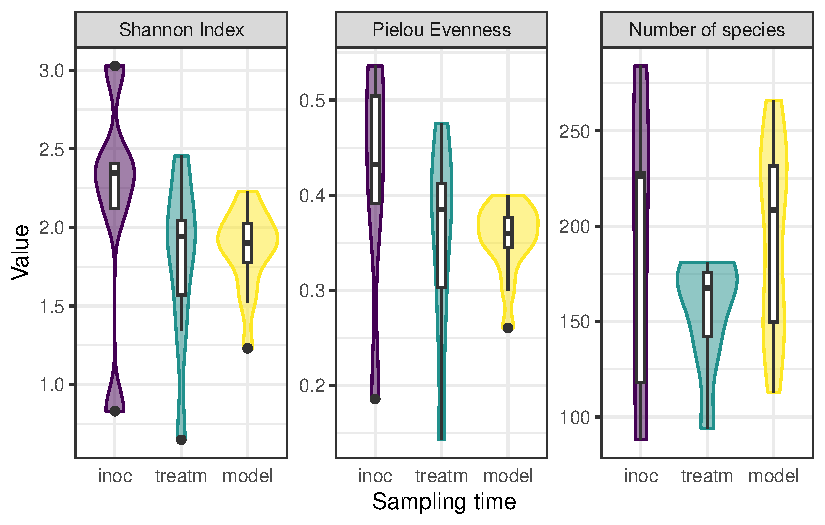
\includegraphics[keepaspectratio]{figures/fig-diversity-byoc-1.pdf}}

}

\caption{\label{fig-diversity-byoc}Plot of Shannon Index, Pielou
Evenness Index, and number of species across experiment samples grouped
by sampling time. inoc = samples from days 0-5; treatm = samples from
days 6-23; model = model calculus samples from day 24.}

\end{figure}%

To monitor the development of microbial communities over the course of
the experiment, we used the Shannon Index to assess the species
diversity and richness at various stages of our protocol. Samples were
grouped into sampling categories due to low sample sizes on sampling
days (inoc = days 0, 3, 5; treatm = days 7, 9, 12, 15; model = day 24).
There was a slight decrease in mean Shannon Index between inoculation
and treatment samples, followed by a slight increase to model calculus
samples, as well as a decrease in variance within sample types. The
Pielou Evenness Index showed a similar pattern while the number of
species increased between the treatment period and the final model
calculus (Figure~\ref{fig-diversity-byoc}).

\paragraph{Medium and model calculus samples are distinct from the
inoculate}\label{medium-and-model-calculus-samples-are-distinct-from-the-inoculate}

\begin{figure}

\centering{

\pandocbounded{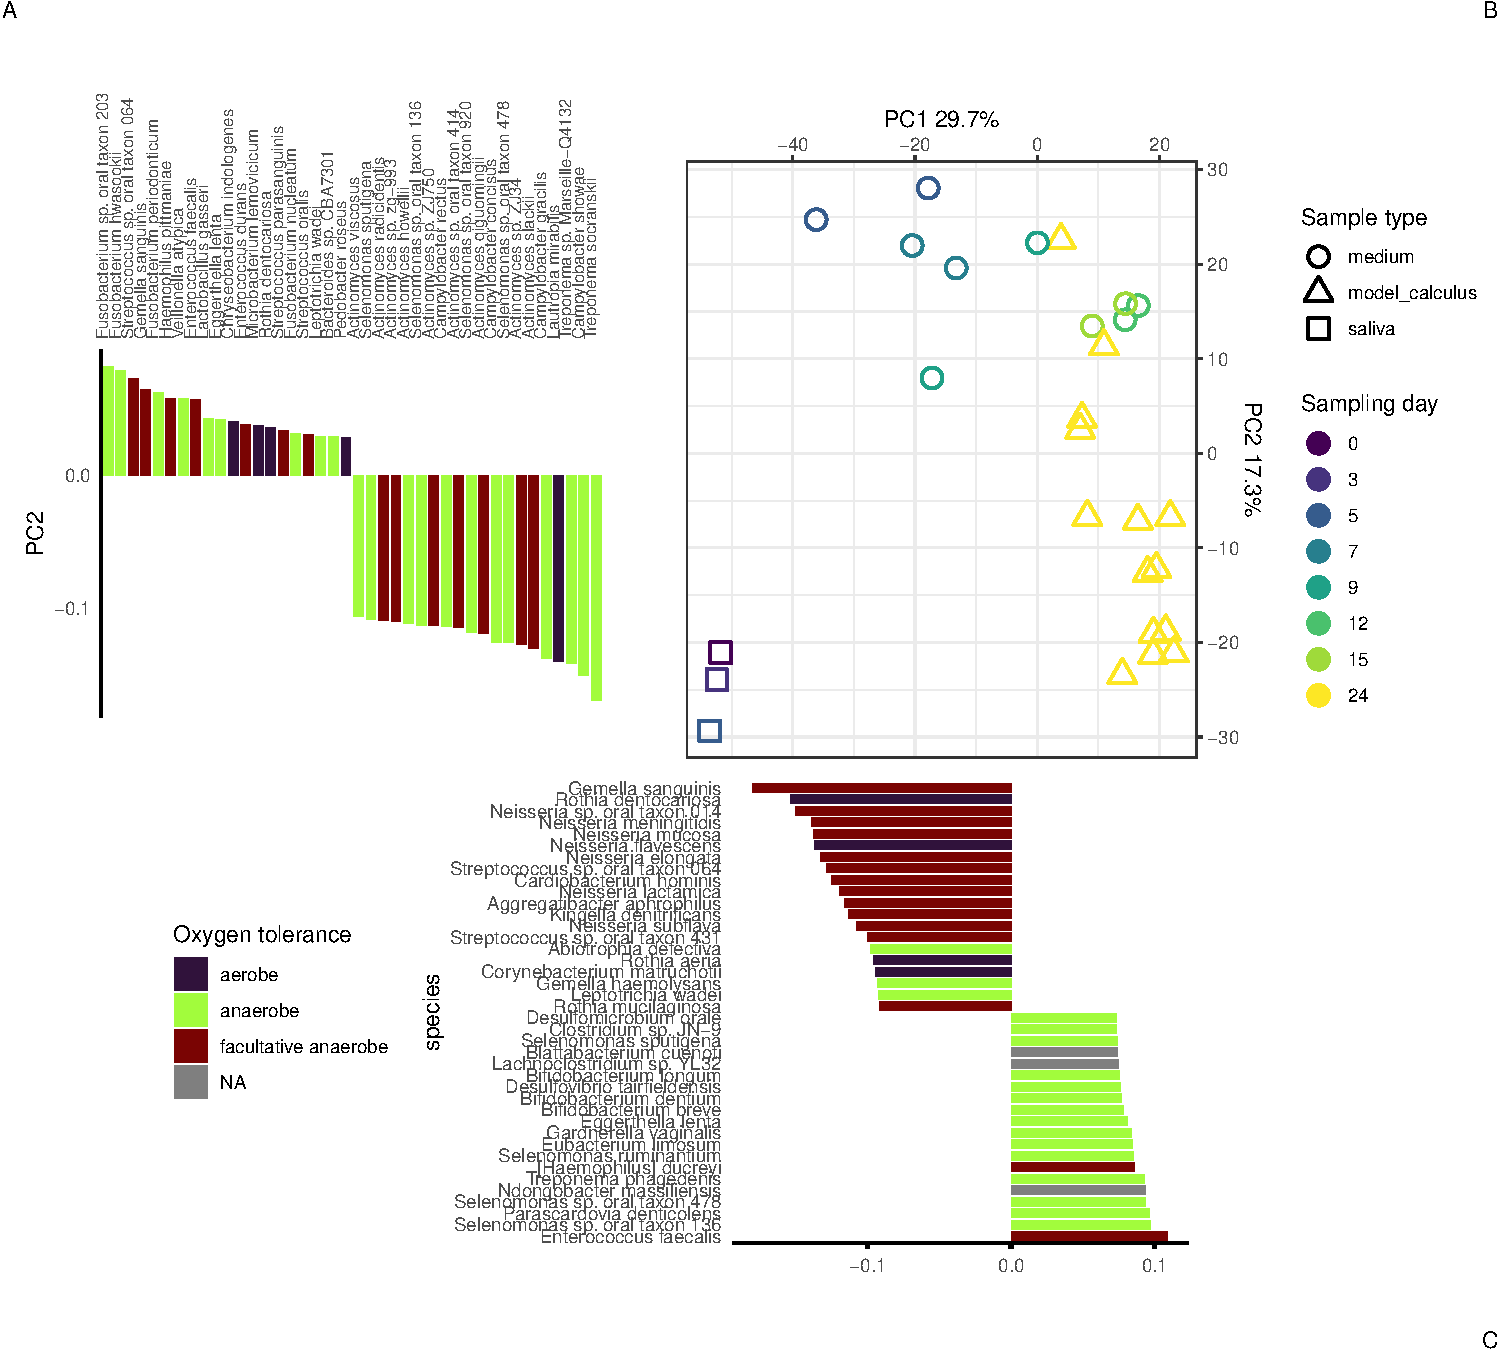
\includegraphics[keepaspectratio]{figures/fig-spca-byoc-1.pdf}}

}

\caption{\label{fig-spca-byoc}sPCA on species-level counts and oxygen
tolerance in samples from this study only. Figure shows the main sPCA
plot (A), species loadings on PC2 (B), and species loadings on PC1 (C).}

\end{figure}%

We next examined whether there is a change in the species composition
over time in our samples by assessing the beta-diversity in a PCA. The
species profiles of the saliva inoculate used in our experiment were
distinct from both medium and model calculus samples. Most of the
separation of saliva from model calculus is on PC1 of the sPCA, where
most of the positive sample loadings are driven by anaerobic species
(model calculus), especially \emph{Selenomonas} spp, and negative
loadings are predominantly facultative anaerobes and some aerobes, such
as \emph{Rothia} and \emph{Neisseria} spp (saliva). Medium and saliva
are separated mostly on PC2, with medium samples located between saliva
and model calculus samples. Model calculus samples also cluster
separately from the medium samples on PC2, with some overlap between the
more mature medium samples and model calculus. Most of the negative
loadings separating saliva and model calculus from medium samples are
dominated by \emph{Actinomyces} spp., while positive species loadings
are more diverse, and seemingly unrelated to aerotolerance
(Figure~\ref{fig-spca-byoc}).

\begin{figure}

\centering{

\pandocbounded{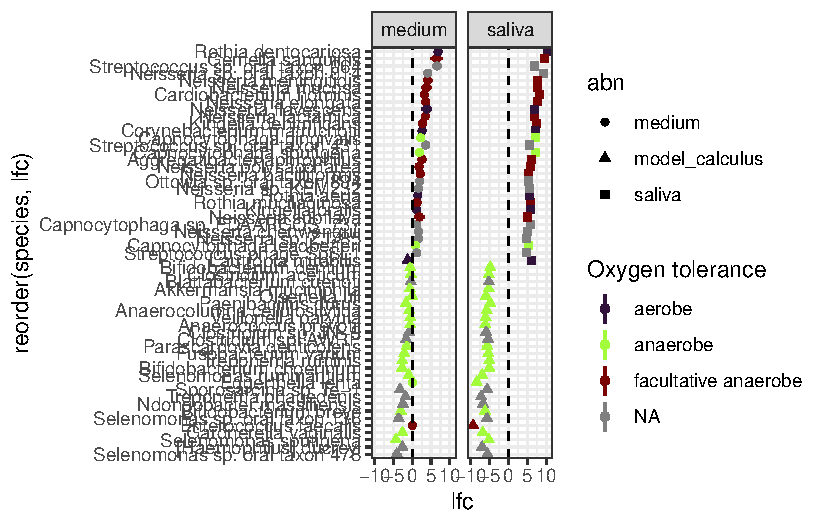
\includegraphics[keepaspectratio]{figures/fig-diffabund-byoc-1.pdf}}

}

\caption{\label{fig-diffabund-byoc}Log-fold changes between sample
types. Circles are species enriched in the medium, triangles are
enriched in model calculus, and diamonds are enriched in saliva. Lines
are standard error. Plot shows the top 30 absolute log-fold changes
between model calculus and saliva.}

\end{figure}%

We determined whether there are species that are differentially abundant
between our sample types using the ANCOMBC R package
\citep{linANCOMBC2020}, giving us an idea of how the biofilm develops
under our experimental conditions. Species enriched in saliva compared
to model calculus are largely aerobic or facultatively anaerobic, while
species enriched in model calculus compared to saliva are mainly
anaerobes. The differences between saliva and calculus are more
pronounced than between medium and model calculus, which is expected
(Figure~\ref{fig-diffabund-byoc}).

\paragraph{Lower diversity in artificial samples than oral
references}\label{lower-diversity-in-artificial-samples-than-oral-references}

\begin{figure}

\centering{

\pandocbounded{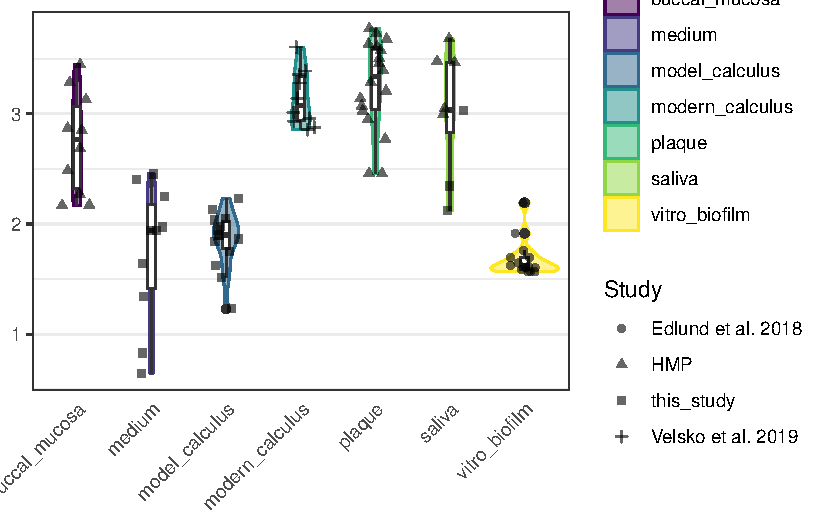
\includegraphics[keepaspectratio]{figures/fig-shannon-compar-1.pdf}}

}

\caption{\label{fig-shannon-compar}Shannon Index for model calculus and
medium samples, as well as oral reference samples and comparative
\emph{in vitro} study.}

\end{figure}%

We used the Shannon Index to compare alpha-diversity in our model to
oral reference samples. The mean Shannon Index of model
samples---medium, model calculus, reference \emph{in vitro} biofilm were
consistently lower than the means of oral reference samples---mucosa,
modern reference dental calculus, saliva, and subgingival and
subgingival plaque. The Pielou species evenness index has a similar
distribution, although the comparative biofilm samples have a higher
mean than biofilm samples from this study. Saliva inoculate samples from
this study have a lower mean Shannon index than reference samples, which
may have contributed to the lower alpha-diversity in model samples
compared to reference samples. The number of species follows the same
trend.

\paragraph{Model calculus is distinct from dental calculus and other
oral
samples}\label{model-calculus-is-distinct-from-dental-calculus-and-other-oral-samples}

\begin{figure}

\centering{

\pandocbounded{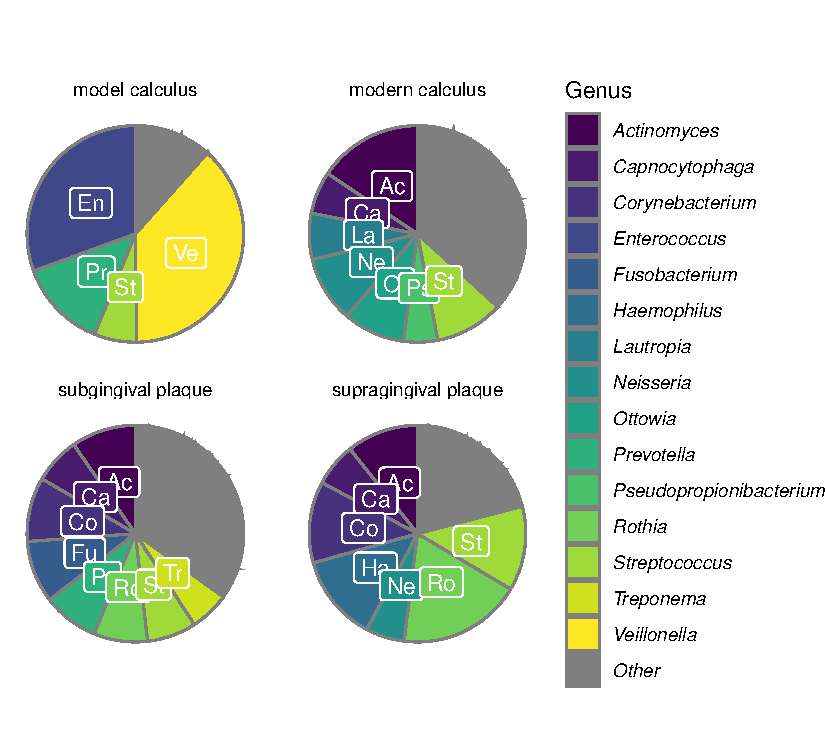
\includegraphics[keepaspectratio]{figures/fig-core-genera-1.pdf}}

}

\caption{\label{fig-core-genera}Core genera within the different types
of samples represented as mean relative abundances at the genus level.
Other = other genera present in lower than 5\% relative abundance.}

\end{figure}%

We calculated the mean relative abundances of the genera in each sample
to compare the core genera of model calculus with oral reference
samples. The most common genera (\textgreater5\% relative abundance) are
shown in Figure~\ref{fig-core-genera}. The main overlap between the
model calculus and oral reference samples is the high relative abundance
of \emph{Streptococcus}. Model calculus consists mostly of
\emph{Enterococcus} and \emph{Veillonella} spp., despite both having low
abundance in donor saliva. \emph{Enterococcus} are also known
environmental contaminants, and we cannot exclude environmental
contamination as a possible source for these species in our model. Oral
reference samples have a more balanced composition, as they are also
represented by fastidious early-coloniser species like
\emph{Capnocytophaga} and \emph{Neisseria} spp., which require an
environment with at least 5\% carbon dioxide to thrive
\citep{tonjumNeisseria2017}.

\begin{figure}

\centering{

\pandocbounded{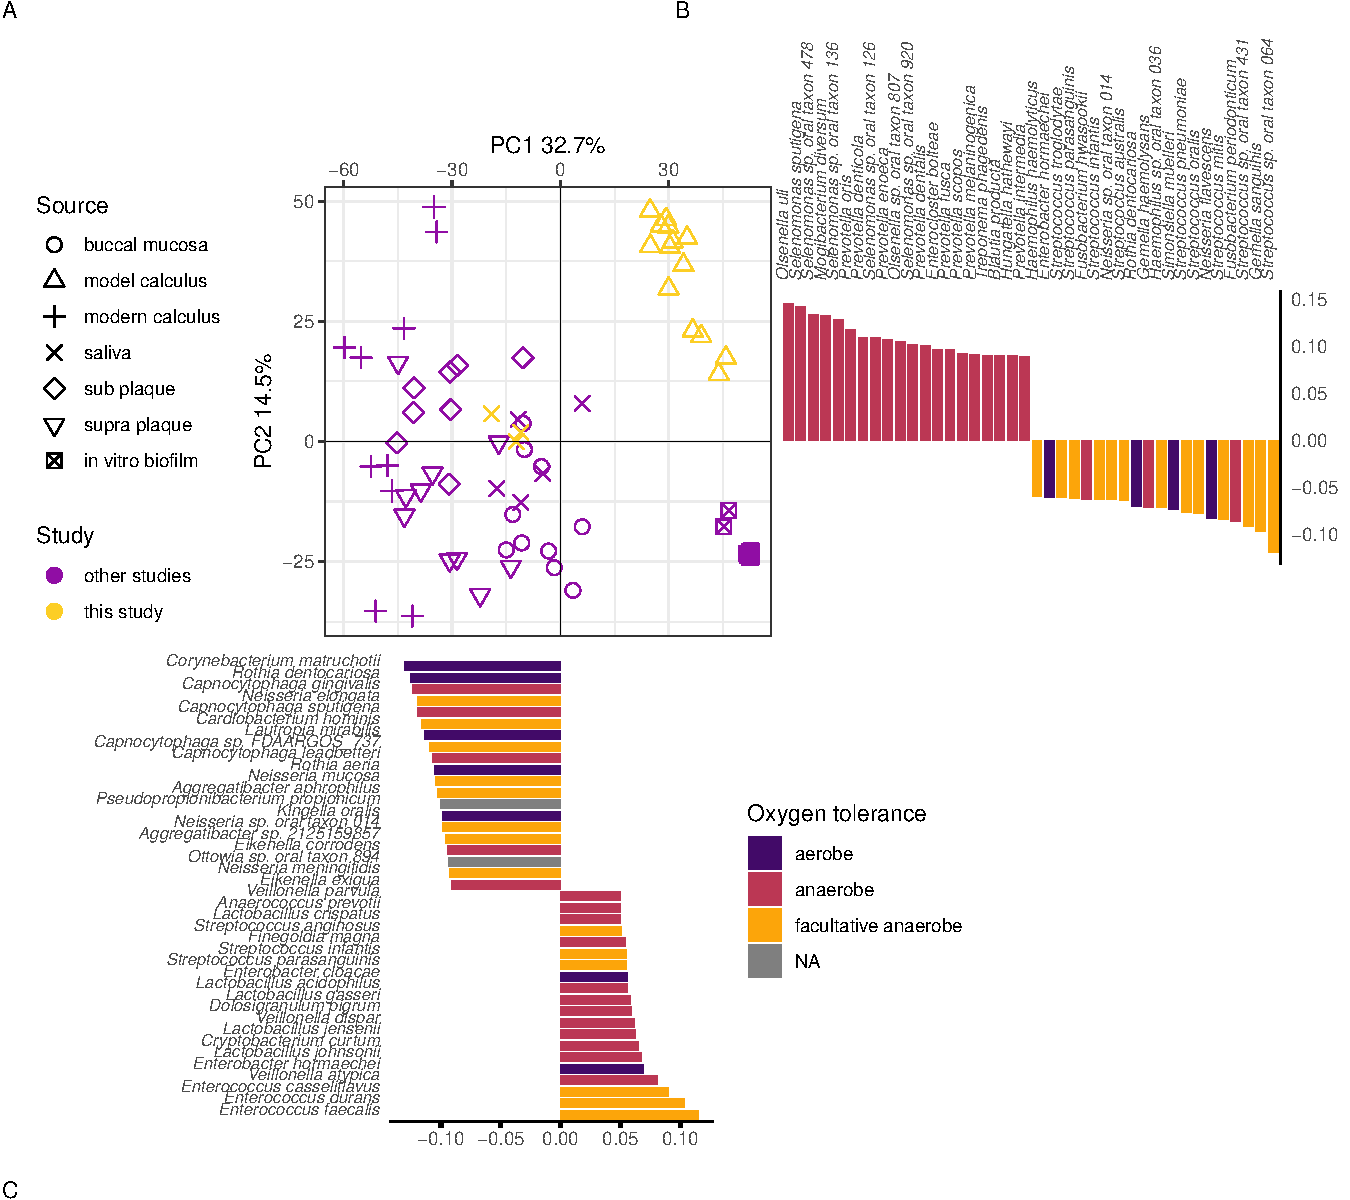
\includegraphics[keepaspectratio]{figures/fig-spca-compar-1.pdf}}

}

\caption{\label{fig-spca-compar}sPCA on species-level counts from model
calculus and reference samples. Figure shows (A) the main sPCA plot, (B)
the species loadings from PC2, and (C) species loadings on PC1.}

\end{figure}%

To directly compare the beta-diversity of our model calculus with oral
reference samples, including modern dental calculus, we used an sPCA
including only our model calculus and reference samples. Model calculus
samples are distinct from both the oral reference samples and the
biofilm model reference samples. They are separated from oral reference
samples mainly on PC1, and from biofilm model reference samples (and, to
some extent, oral samples) on PC2. The highest negative contributions
are a mix of all types of aerotolerance, while the positive
contributions are mostly (facultative) anaerobes, with
\emph{Enterococcus} spp. as the top three positive contributors to PC1.
Top negative contributors are \emph{Capnocytophaga} spp as well as the
aerobes \emph{Corynebacterium matruchotii} and \emph{Rothia
dentocariosa}. The top positive contributors to PC2 are all anaerobes,
mainly from the genus \emph{Selenomonas}. Top negative contributors to
PC2 are a mix of aerotolerances, with many \emph{Streptococcus} spp
(Figure~\ref{fig-spca-compar}).

\begin{figure}

\centering{

\pandocbounded{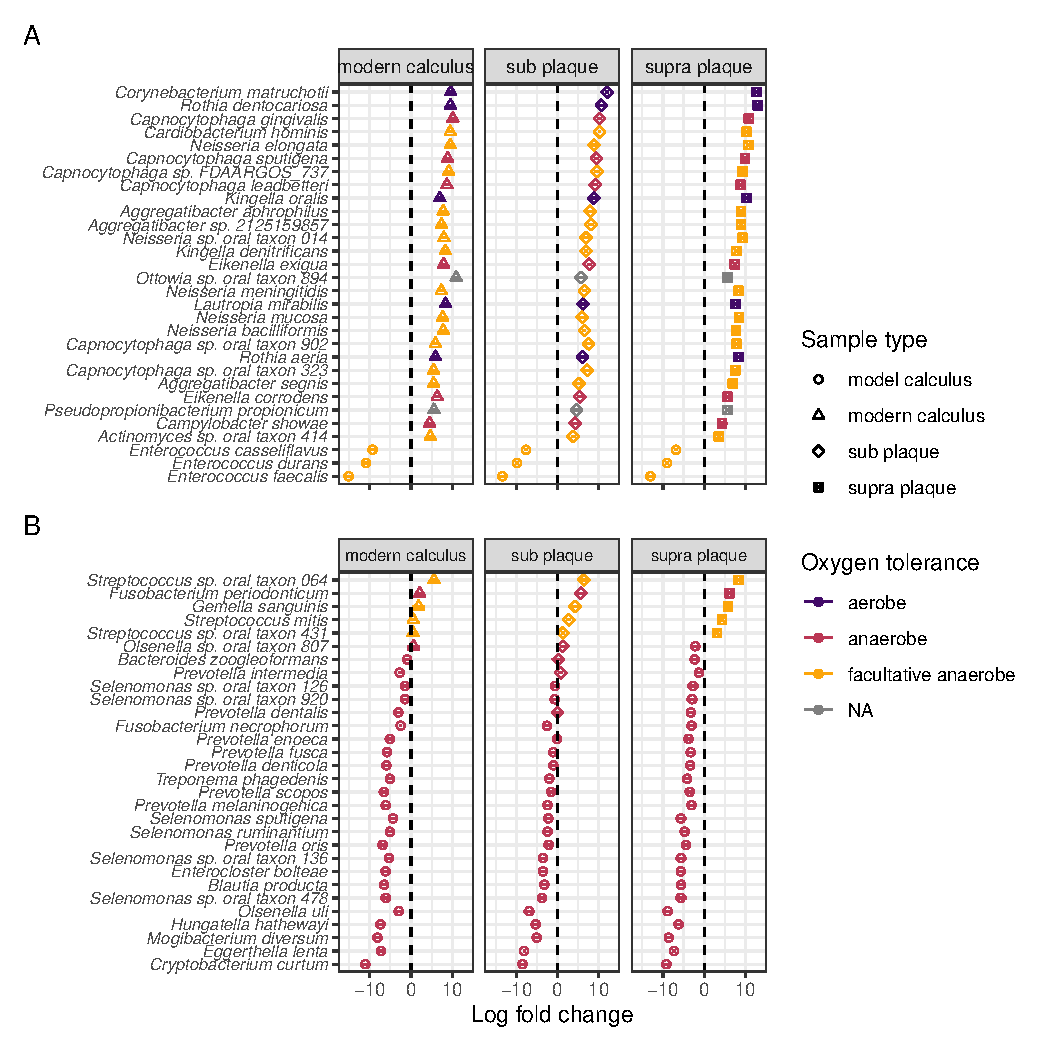
\includegraphics[keepaspectratio]{figures/fig-diffabund-comp-1.pdf}}

}

\caption{\label{fig-diffabund-comp}Log-fold changes between sample
types. Circles are species enriched in the model calculus, triangles in
modern calculus, diamonds are enriched in subgingival plaque, and
squares in supragingival plaque. Plot shows the top 30 loadings
(absolute value) in PC1 (A) and PC2 (B) between model calculus and other
sample types, ordered by decreasing log-fold change. Bars represent
standard error.}

\end{figure}%

To investigate which species are enriched in different sample types, and
compare the final product of our model with naturally occurring plaque
and calculus samples, we performed differential abundance analysis on
our model calculus samples, modern dental calculus, and sub- and
supragingival plaque. Based on the differential abundance analysis the
main differences between model calculus and oral reference samples, when
looking at the top 30 contributors to PC1, are that the oral reference
samples are enriched with species with a diverse oxygen tolerance from a
wide range of genera, while the model calculus is enriched with
\emph{Enterococcus} spp. The largest differences occur in
\emph{Corynebacterium matruchotii}, \emph{Rothia dentocariosa}, and
\emph{Capnocytophaga gingivalis} (Figure~\ref{fig-diffabund-comp}A).
This is echoed when looking at the top 30 contributors to PC2, where
most of the species are enriched in model calculus, all of which are
anaerobes, and the largest differences occurring in
\emph{Cryptobacterium curtum}, \emph{Eggerthella lenta}, and
\emph{Mogibacterium diversum} (Figure~\ref{fig-diffabund-comp}B).

\subsubsection{Samples show an increased mineralisation over the course
of the
experiment}\label{samples-show-an-increased-mineralisation-over-the-course-of-the-experiment}

To determine whether the model dental calculus is comparable to natural
dental calculus, both modern and archaeological dental calculus were
analysed with FTIR spectroscopy to ascertain their composition.

It is evident that between days 7 and 24 there is a decrease of the
protein components and increase of the inorganic mineral carbonate
hydroxyapatite. The model calculus samples from the end of the
experiment are similar to both the modern and archaeological reference
samples. The main difference is a lower organic component in reference
samples seen as a reduced amide I peak at around 1637 compared to the
carbonate peak at around 1420, and an absence of amide II and III.
Further, there is a reduction in CH3 bands at 3000-2900 cm\(^{-1}\)
(Figure~\ref{fig-ftir-spectra}A-D).

Sample spectra from days 7 and 12 are characterised by a high content of
proteins as evident by the strong amide I absorbance band at 1650, a
less pronounced amide II band at 1545 cm\(^{-1}\), and the small amide
III band at 1237 cm\(^{-1}\). Related to the organic component of the
samples are also the three marked CH\textsubscript{3} and
CH\textsubscript{2} stretching vibrations at 2960, 2920, and 2850
cm\(^{-1}\) wavenumbers. The presence of mineral component is evident
from the presence of C--O\(^{2-}_3\) absorbance bands at 1450 and 1400
cm\(^{-1}\) wavenumbers typical of carbonates, and P--O\(^{3-}_4\)
absorbance band at 1080 and 1056 cm\(^{-1}\) which are related to
phosphate minerals. There is a large variation between the spectra,
possibly indicating different formation rates of the different
components in the samples (Figure~\ref{fig-ftir-spectra}A and B).

In spectra from days 16 to 24, the ratio of amides to
PO\textsubscript{4} has shifted, with the main peak shifting to the
PO\textsubscript{4} v\textsubscript{3} absorbance band at 1039--1040
cm\(^{-1}\), indicating that the main component of the samples is
carbonate hydroxyapatite. A well-defined PO\textsubscript{4} doublet at
600 and 560 is present. Small CO\(_3^{2-}\) asymmetric stretching at
1450 cm\(^{-1}\) and 1415 cm\(^{-1}\), and stretching vibrations at
875-870 cm\(^{-1}\) indicate that the carbonate minerals component is
also becoming more crystallised. There is a decreased variability
between the spectra, with most spectra exhibiting a higher
phosphate-to-protein/lipid ratio (Figure~\ref{fig-ftir-spectra}C and D).

\subsubsection{Model calculus has a similar mineral composition to
natural
calculus}\label{model-calculus-has-a-similar-mineral-composition-to-natural-calculus}

Archaeological and modern reference spectra are largely
indistinguishable and consist of a broad O--H absorbance band (3400
cm\(^{-1}\)) related to amid a and hydroxyl group, weak CH3 bands
(3000--2900 cm\(^{-1}\)), amide I band (1650 cm\(^{-1}\)) which is
related to the protein content, carbonate (1420, 1458-1450, 875-870
cm\(^{-1}\)), and phosphates (1036-1040, 602-4, 563-566 cm\(^{-1}\))
(Figure~\ref{fig-ftir-spectra}E) which, together with the hydroxyl and
the carbonate, can be identified as derived from carbonate
hydroxyapatite, the main mineral found in mature dental calculus
\citep{hayashizakiSiteSpecific2008, jinSupragingivalCalculus2002}.

\begin{figure}

\centering{

\pandocbounded{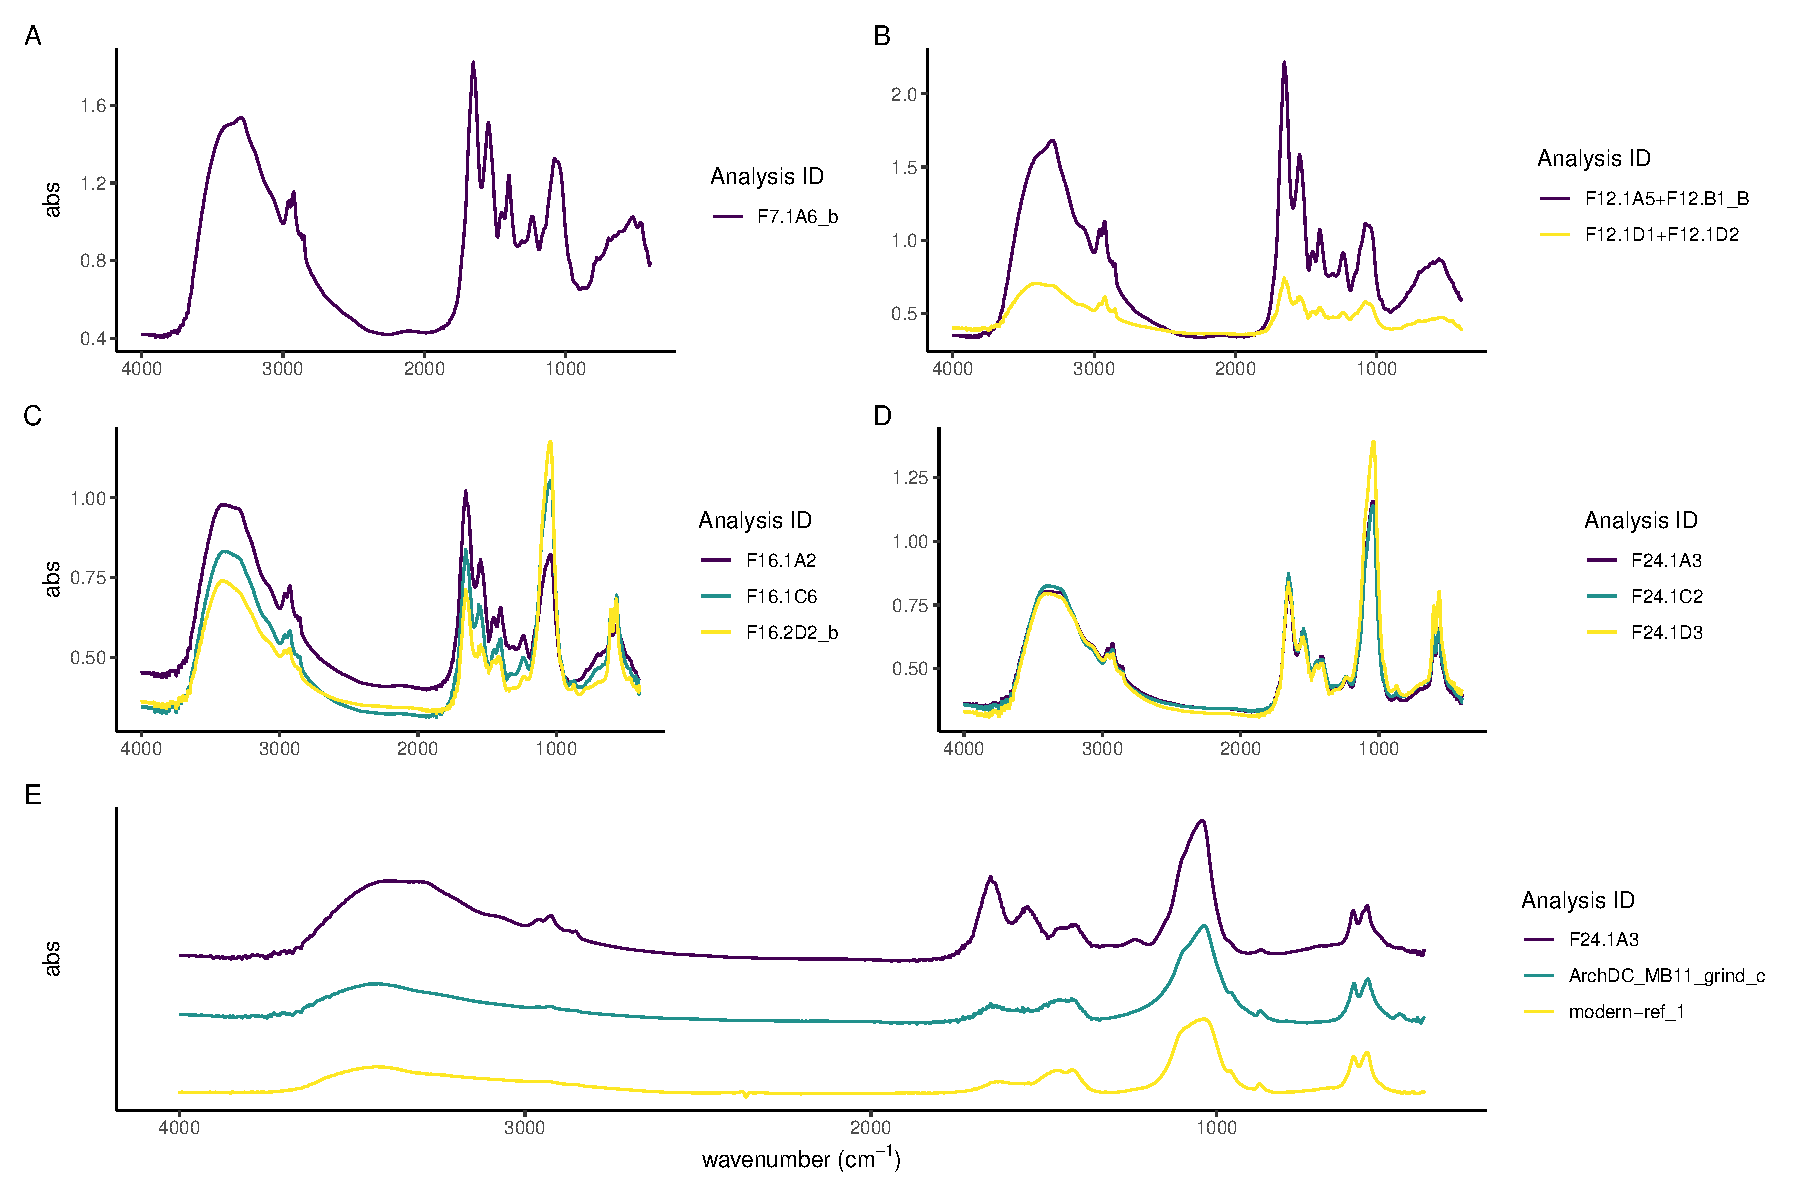
\includegraphics[keepaspectratio]{figures/fig-ftir-spectra-1.pdf}}

}

\caption{\label{fig-ftir-spectra}Select spectra from all experiment
sampling days; (A) day 7, (B) day 12, (C) day 16, and (D) day 24.
Absorbance bands in stretching mode around 3400 cm−1 typical of the
hydroxyl group. Analysis ID for model samples is constructed as: F{[}day
sampled{]}.{[}well sampled{]}\_{[}grind sample{]}.}

\end{figure}%

\subsubsection{Samples show similar crystallinity and order to reference
calculus}\label{samples-show-similar-crystallinity-and-order-to-reference-calculus}

We determined the level of crystallinity and order of the carbonate
hydroxyapatite in our samples as an indication for its maturity by using
the grinding curves method presented by
\citet{asscherAtomicDisorder2011} and
\citet{asscherVariationsAtomic2011}.\\
Samples were compared to published trendlines for archaeological and
modern enamel \citep{asscherAtomicDisorder2011}. We see no appreciable
differences between days 16, 20, and 24. The archaeological dental
calculus shows a slightly increased slope compared to model calculus
from the three sampling days used in the grind curve
(Figure~\ref{fig-grind-curve}), possibly indicating larger crystal size
due to more complete crystalisation. The steeper slope of enamel samples
is consistent with a more ordered structure in enamel compared to dental
calculus.

\begin{figure}

\centering{

\pandocbounded{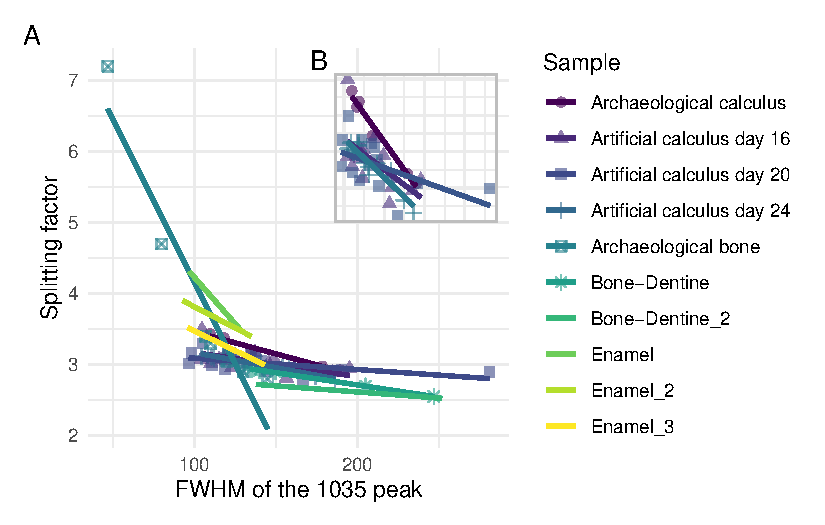
\includegraphics[keepaspectratio]{figures/fig-grind-curve-1.pdf}}

}

\caption{\label{fig-grind-curve}Grinding curves of our biofilm and model
calculus compared to published trendlines (dashed light grey lines) for
archaeological (dotted line) and modern (dashed line) enamel.}

\end{figure}%

\section{Discussion}\label{discussion}

In this study we present a calcifying oral biofilm model to produce
artificial dental calculus. Our proposed use of the model is to address
a variety of research questions related to dietary information extracted
from dental calculus, in both modern and archaeological samples. For
that to be feasible, the model needs to serve as a viable proxy to
dental calculus grown under natural conditions, i.e., in the human oral
cavity. It needs, as much as possible, to mimic the diversity and
complexity of the natural oral microbiome, while also offering control
over factors such as dietary input, growth conditions, and replicability
within and between experiments. Here, we assessed the viability of our
model as a proxy for dental calculus using metagenomic classification
and FTIR analysis to explore the bacterial and mineral composition, and
compare with oral reference samples.

\subsubsection{Microbiome}\label{microbiome}

Model calculus has lower species diversity than inocula saliva and oral
reference samples, which is a common limitation in biofilm models
\citep{edlundBiofilmModel2013, bjarnsholtVivoBiofilm2013}. The donated
saliva for the experiment had a lower diversity than the reference
saliva samples, and may have contributed to a lower diversity in
experimental samples. Consequently, there is also a lower diversity and
richness when compared to other modern oral reference samples, including
oral mucosa, saliva, plaque, and calculus. Samples of the medium from
early in the experiment have similar species profiles to the donated
saliva, but gradually diverge over the course of the experiment. This
may be caused by experimental setup not sufficiently mimicking the oral
environment, allowing species to thrive that do not normally thrive in
the natural oral environment.

Oral reference samples have a relative abundance of streptococci similar
to our model, but a more diverse representation from other genera and an
overall higher species diversity and richness than our model. Reference
samples also had a more diverse aerotolerance profile than our model,
which primarily consisted of (faculatative) anaerobes. Species within
predominantly aerobic genera, are deficient in the model, suggesting a
shift from a largely aerotolerant profile to an anaerobic profile during
the experiment. While our model is not set up as an anaerobic system,
the anaerobes seem to have outcompeted aerobes and, to some extent,
facultative anaerobes. This is likely a result of communities of
bacteria within the biofilm creating favourable microenvironments
facilitated by the protective properties of the biofilm matrix
\citep{flemmingBiofilmsEmergent2016, edlundUncoveringComplex2018}.

Overall, the majority of model calculus samples contained a distinctly
oral signature, providing a promising starting point for the use of the
model as a viable proxy to dental calculus. The main differences between
model and oral reference samples may be due to human variation, as there
can be large differences in the oral microbiome of two individuals at
the species level due to variations in age, sex, and other demographic
factors, as well as how and when saliva samples were collected
\citep{burchamPatternsOral2020, nearingAssessingVariation2020}. Whether
or not distinct microbial profiles, and the extracellular matrix they
produce, will affect the retention of dietary particles in plaque
remains to be seen, but is an important question to address in the
future.

\subsubsection{Mineralisation}\label{mineralisation}

FTIR analysis allowed us to address the mineralisation process of the
model, which showed an increasing mineral composition over the course of
the experiment. As the model biofilm matured, the predominantly organic
content of early samples was replaced by inorganic content in the form
of carbonated hydroxyapatite, consistent with a shift from a high
presence of bacterial cells in a matrix of extracellular polysaccharides
\citep{jainIsolationCharacterization2013, sutherlandBiofilmMatrix2001, zhangMeasurementPolysaccharides1998}
to a predominantly mineral content.

The model calculus samples resemble both the modern reference calculus
and the archaeological calculus in mineral composition and
crystallinity. The steeper slope in the grind curve plots of the
archaeological sample suggests that the crystals in archaeological
samples are larger, and hence more ordered than in model calculus. A
possible explanation is that the inorganic crystals within
archaeological calculus have had more time to grow into the space left
by degraded organic matter \citep{weinerBiologicalMaterials2010};
however, we only analysed one archaeological sample and cannot
definitively address this. The short duration of model calculus growth
may also have affected the results, compared to the longer-term growth
and mineralisation of natural calculus. The constant disruptions in
growth of \emph{in vivo} dental plaque/calculus, due to oral hygiene and
other external pressures on biofilm growth, may lead to multiple stages
of calcium phosphates, whereas our model has more stable growth
conditions.

One of the most well-known biomineralisers, \emph{Corynebacterium
matruchotii}
\citep{enneverCharacterizationBacterionema1978, takazoeCalciumHydroxyapatite1970},
exhibited a lower abundance in our model calculus compared to modern
reference calculus. However, the mineral composition of the end results
were similar, reinforcing the idea that, under the right circumstances,
biofilms with a range of microbial profiles can facilitate
mineralisation \citep{moorerCalcificationCariogenic1993}. Bacteria and
their ability to secrete an extracellular matrix are integral in the
formation of dental calculus, and inevitably serve as part of the
structure that dental calculus is built upon
\citep{rohanizadehUltrastructuralStudy2005}, while the exact species
composition of the biofilm communities may be less important.

\subsubsection{Replicability}\label{replicability}

Model calculus displayed similar species diversity and microbial
profiles across all samples, indicating a high level of replicability
between samples in the experimental run. It remains to be seen whether
the replicability within the experiment also scales up to
between-experiment replicability in our model, though others have
already shown that replicability in long-term models is possible when
using the same inocula \citep{velskoConsistentReproducible2018}. The
variation in mineral composition in our model was initially high, but
samples from day 24 were largely similar in composition as observed in
the FTIR spectra. The use of a simple multiwell plate setup allows us to
submit many samples to the same conditions, increasing replicability
between samples \citep{extercateAAA2010}.

\subsubsection{Limitations}\label{limitations}

While our in vitro model calculus system provides reproducible and
consistent artificial dental calculus for archaeological research, as
demonstrated by the species composition and the mineralisation
properties, we recognise the model has several limitations. Our
single-donor approach may have affected the diversity of the model. The
donated saliva from our study had a lower mean Shannon Index than other
saliva samples. The lower diversity may be caused by only using one
donor instead of pooling saliva from multiple individuals. However,
having a single inoculum donor allows us to maintain the integrity of a
native oral microbiome which may be lost when samples are pooled
\citep{edlundBiofilmModel2013}. It is also possible that the diversity
was affected by the collection and storage methods we used. This has
been shown to have minimal effect on microbial profiles at the genus
level \citep{limSalivaMicrobiome2017}, but some effect on beta diversity
calculations \citep{omoriComparativeEvaluation2021}.

Some samples were grown with starch-sucrose solutions as nutrients,
while controls were grown with sucrose only. Due to the financial cost,
we did not sequence enough samples of each nutrient treatment to assess
the influence of starch on the microbial community or mineral
composition. Biofilms were grown in a standard shaking bacterial growth
incubator, rather than an incubator specific to cell cultures. The lack
of complex environmental control may cause the model to deviate from its
natural growth over the 25 days that the experiment is run, due to a
lack of precise control over conditions such as pH and salivary flow
rates.

There is also the possibility that contamination was introduced into the
model during the experiment. While the CPMU solution was prepared under
sterile conditions, the solution itself was not autoclaved or
filter-sterilised. In the species composition metagenomic analysis, all
medium samples collected after the introduction of CPMU on day 14 were
removed by the authentication step because the majority of species
appeared to derive from environmental sources indicating external
contamination. Going forward we recommend filter-sterilising solutions
that are not autoclaved.

To avoid disturbing the growth and development of our biofilm, we took
samples of media from the bottom of the wells after three days without
full media replacement, careful not to disturb other plate-bound
biofilms. The samples may therefore not fully reflect the composition of
the biofilm itself. Going forward we recommend sampling from the actual
biofilm, as this is the sample type under investigation.

\subsubsection{Future work}\label{future-work}

Further protocol optimisation will also be necessary to address some of
the limitations of our current model, such as reducing the frequency of
medium replacement (currently every three days) to help promote the
growth of slow-growing fastidious organisms and limit generalists such
as enterococci, and supplementing it with serum to provide additional
nutrients and biofilm stability
\citep{tianUsingDGGE2010, ammannZurichBiofilm2012}. More infrequent
medium replacement would facilitate slow-growing bacteria in
establishing their metabolic relationships, allowing the byproducts of
some species to become abundant enough for others that depend on these
to grow \citep{marshDentalPlaque2005}.

Our goals for additional validation measures involve functional profiles
of bacteria, to see if metabolic behaviour of bacteria is consistent
with \emph{in vivo} conditions, and whether this is affected by the
presence/absence of amylase and starch treatments. The absence of host
salivary \(\alpha\)-amylase activity in our model (as shown in
\citet{bartholdyInvestigatingBiases2022}) provides an opportunity to
explore the effect of various amylase levels on biofilm growth and
composition, as well as the incorporation of dietary compounds in dental
calculus.

The model can also be used to explore limitations and biases of methods
used to reconstruct past dietary patterns from dental calculus. To this
end, sucrose and raw starch treatments can be replaced with other
dietary components of interest, such as cooked starches, whole plant
extracts, and various proteins.

\subsection{Conclusions}\label{conclusions}

The bacterial profile of our model calculus is not an exact match to the
natural modern or archaeological reference calculus, but species
richness and diversity falls within a similar range as the reference
\emph{in vitro} model, and the core genera are predominantly oral. Our
model calculus had a distinct microbial profile from modern reference
calculus, but a similar mineral composition to modern and archaeological
reference calculus, consisting of carbonate hydroxyapatite and similar
levels of crystallinity and order, with a slightly higher organic phase.

Our model has many potential benefits within archaeological research,
especially since the setup does not require highly specialised
equipment, making it accessible to many labs within the archaeological
sciences. It can be used to test many fundamental aspects of the process
of incorporation, retention, and subsequent extraction of various
dietary components from archaeological dental calculus. Using an oral
biofilm model in a controlled environment with known dietary input, we
can learn more about how different methods of food processing in the
past may affect results of dental calculus analyses, and how the methods
we use may further distort this picture. Our method can be used to test
methods (e.g.~DNA, proteomics, etc.), decontamination protocols, as well
as training on these methods and protocols without depleting limited
archaeological resources. The purpose of our model is not to replace
studies conducted on archaeological and natural dental calculus, but
rather to balance limitations of each method and serve as a
complementary approach to expand our toolkit.

\section*{Acknowledgements}\label{acknowledgements}
\addcontentsline{toc}{section}{Acknowledgements}

We would like to thank the nf-core/eager community for assistance with
the EAGER pipeline, especially Dr.~James Fellows Yates. We also thank
Sophie Seng for involvement in the DNA extraction. This work was
performed using the compute resources from the Academic Leiden
Interdisciplinary Cluster Environment (ALICE) provided by Leiden
University, with special thanks to Dr.~Robert Schulz. The FTIR analysis
was conducted at the Laboratory for Sedimentary Archaeology, Haifa
University, courtesy of Prof.~Ruth Shahack-Gross, with additional help
from Dr.~Yotam Asscher.

This research has received funding from the European Research Council
under the European Union's Horizon 2020 research and innovation program,
grant agreement number STG--677576 (``HARVEST'', funding BPB and AGH),
as well as STG-948365 (``PROSPER'', funding ZF), and Werner Siemens
Foundation (``PALEOBIOTECHNOLOGY, funding IMV and CW).

\section*{Data Availability
Statement}\label{data-availability-statement}
\addcontentsline{toc}{section}{Data Availability Statement}

Human-filtered DNA sequencing data have been deposited in the ENA
database under accession
\href{https://www.ebi.ac.uk/ena/browser/view/PRJEB61886}{PRJEB61886}.
Analysis scripts and source code for the manuscript and supplementary
materials are available on GitHub
(\url{https://github.com/bbartholdy/byoc-valid}) and archived on
4TU.ResearchData
(\href{https://doi.org/10.4121/99932661-fe79-4f4e-a812-a8917ad18fd0}{10.4121/99932661-fe79-4f4e-a812-a8917ad18fd0}).
FTIR data and spectra are available on 4TU.ResearchData
(\href{https://doi.org/10.4121/466b2588-9689-4d84-a8a0-5216aa39e40b}{10.4121/466b2588-9689-4d84-a8a0-5216aa39e40b}).
Detailed protocols for growing the oral biofilm are available on
protocols.io
(\href{https://dx.doi.org/10.17504/protocols.io.dm6gpj9rdgzp/v1}{10.17504/protocols.io.dm6gpj9rdgzp/v1}).

\section*{References}\label{references}
\addcontentsline{toc}{section}{References}

\renewcommand{\bibsection}{}
\bibliography{references.bib}

\end{document}
